% !TEX root = ../../prj4projektrapport.tex
% SKAL STÅ I TOPPEN AF ALLE FILER FOR AT MASTER-filen KOMPILERES 


\section{Interne blokdiagramer}

Herunder ses de interne blokdiagrammer for spændingsregulator systemet. De interne blokdiagrammer er dannet for at give et indtryk af hvordan enhederne kommunikerer og sender signaler indbyrdes. Først ses det interne blokdiagram for hele systemet, hvor de overordnede forbindelser i spændingsregulatoren kan ses. Se figur \ref{fig:IBDSp}. For et yderligere overblik over de indbyrdes signaler, se dokumentation\footnote{Projektdokumentation, 5.2, Intern blok diagram}.  Derefter ses et internt blokdiagram for selve styringsenhed, der yderligere består af tre mindre dele. 

\begin{figure}[htbp] % (alternativt [H])
	\centering
	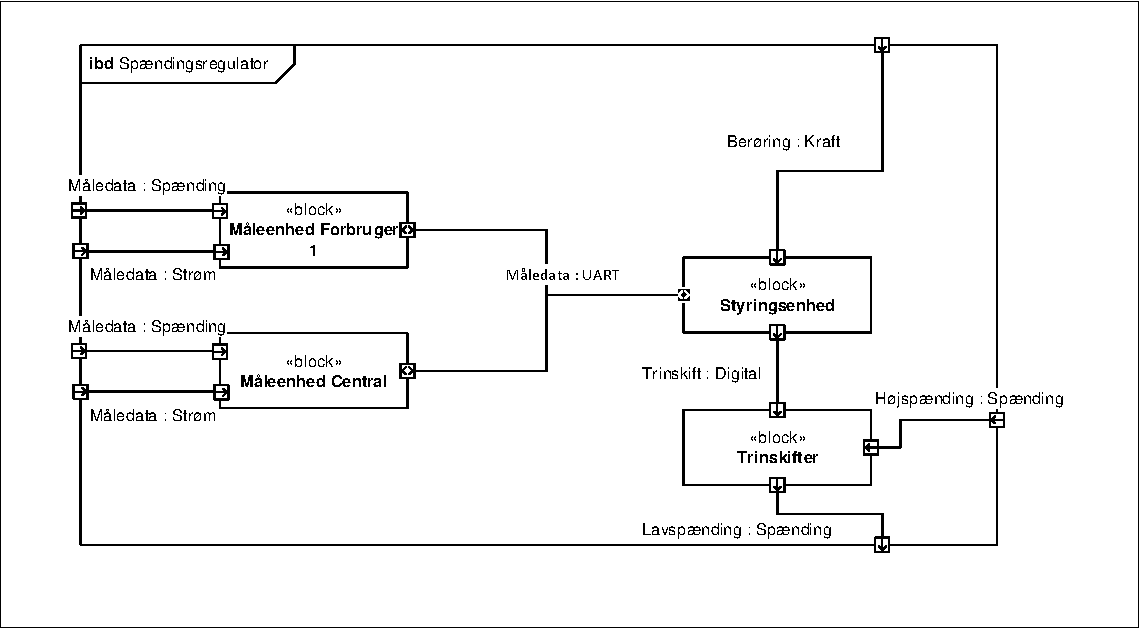
\includegraphics[width=0.8\textwidth]{figure/IBDSpaendingsregulator.pdf}
	\caption{IBD for Spændingsregulator}
	\label{fig:IBDSp}
\end{figure}

Det interne blokdiagram for styringsenheden er udviklet for at beskrive hvordan modulerne i styringsenheden kommunikerer indbyrdes. Det ses samtidig hvilke inputs og outputs der er til og fra den samlede styringsenhed. Se figur \ref{fig:IBDSp}. For yderlig uddybelse af de indbyrdes signaler se dokumentation\footnote{Projektdokumentation, 5.2, Intern blok diagram}.


\begin{figure}[htbp] % (alternativt [H])
	\centering
	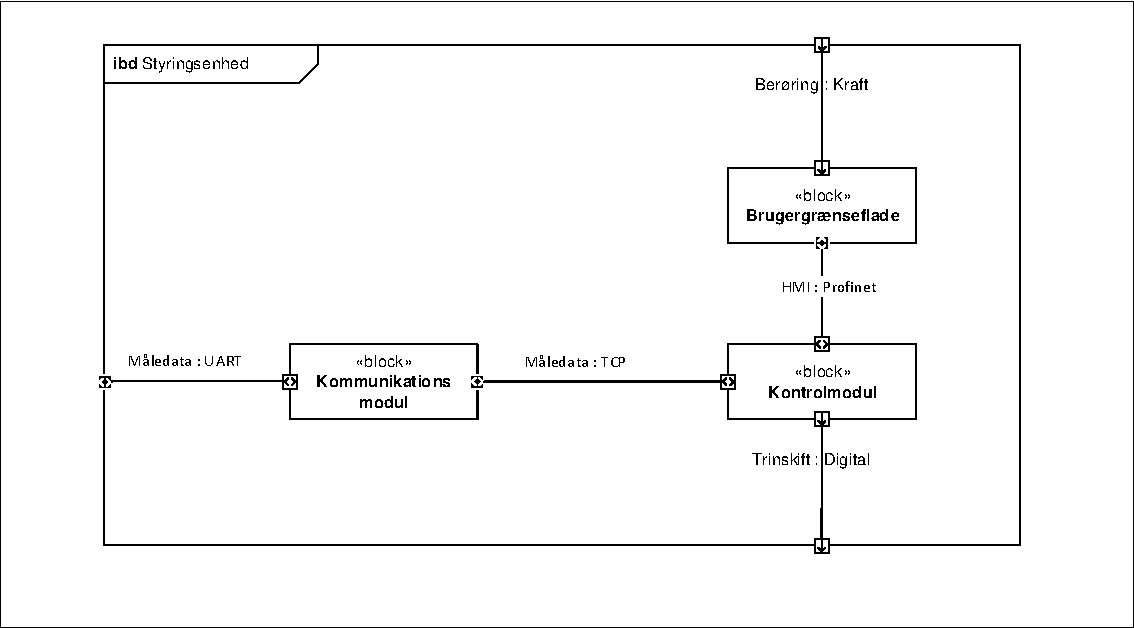
\includegraphics[width=0.8\textwidth]{figure/IBDStyringsenhed.pdf}
	\caption{IBD for Styringsenhed}
	\label{fig:IBDSt}
\end{figure}




